\section{Method}
\label{sec:method}
In this section the method that is being used in the report will be explained.
Firstly the preprocessing of the social network graph will be discussed.
Afterwards the exact elements that we used for the genetic algorithm will be explored.
In total this chapter should give the information required to easily follow section \ref{sec:implementation} where the exact implementation of these methods will be further described.

\subsection{Graph Reduction}
For the preprocessing of the graph we go through several steps.
First of all a random selection will be made of vertices.
Afterwards we look for cliques around these vertices.
Finally we reduce the clique to a single node with additional information.
The result of this step is that the search space is reduced.

Vertices are selected on a random basis but with certain constraints.
A vertices that was used in the creation of a clique will not be considered.
The reasoning behind this constraint is that too much information will be lost if we start creating cliques with other cliques in them.
An example of this can be seen in Fig. \ref{fig:clique}

\begin{figure}[H]
\begin{center}
\begin{tabular}{ccccc}
\raisebox{-.5\height}{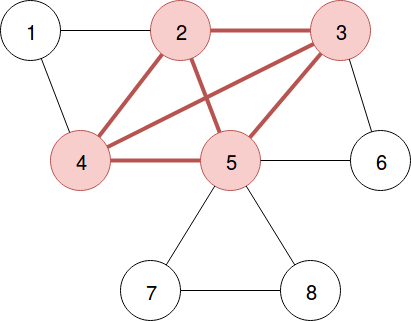
\includegraphics[width=0.25\textwidth]{images/clique.png}} & $\: \rightarrow \:$ & \raisebox{-.5\height}{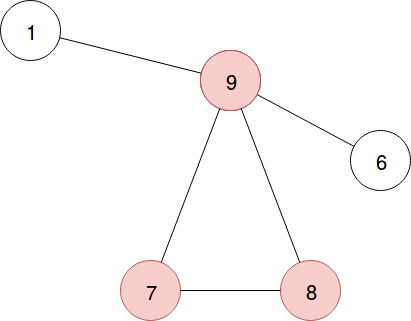
\includegraphics[width=0.25\textwidth]{images/firstReduce.png}} & $\: \rightarrow \:$ & \raisebox{-.5\height}{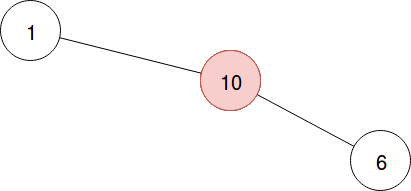
\includegraphics[width=0.25\textwidth]{images/secondReduce.png}}
\end{tabular}
\caption{A clique (left) can yet again be part of a clique (middle) after reduction. This would lead to the rightmost graph, which is no longer a good representation of the structure of the original graph (left).}\label{fig:clique}
\end{center}
\end{figure}

The search for cliques is rather straightforward.
After a vertex is selected (under the constraints) we depth-first search is done.
For every neighbour the vertex has it is checked that if these are added together a complete graph is created by these vertices and thus being a clique.
This process repeats itself until adding a new vertex no longer leads to having a clique.
Then the algorithm will backtrack to find all of the remaining cliques surrounding the originally selected vertex.

\begin{figure}[H]
\begin{center}
\begin{tabular}{ccc}
\raisebox{-.5\height}{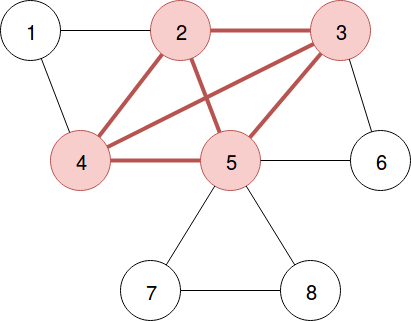
\includegraphics[width=0.30\textwidth]{images/clique.png}} & $\: \rightarrow \:$ & \raisebox{-.5\height}{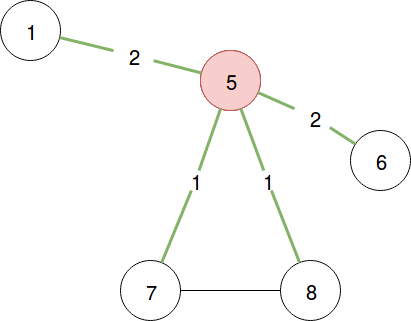
\includegraphics[width=0.30\textwidth]{images/reduced.png}}
\end{tabular}
\caption{The reduction of a clique to a single vertex and the adjustment of weights.}\label{fig:reduction}
\end{center}
\end{figure}

When all of the cliques surrounding a single vertex are found, the largest of them all will be selected for reduction.
With reduction it is meant that the vertices in the clique will be replaced by a single vertex in the graph.
But the underlying information of the edges will be retained by changing the value of the weigths on the corresponding edges.
The edges of which the weights will be adapted are those who are neighbouring to the vertices in the clique as can be seen in Fig. \ref{fig:reduction}.
Edges that have not been affected by any reduction will be considered to have the value of $1$ without explicitly stating it.

The result is a smaller graph.
If there are more edges between the vertices, then the probability of finding a clique also increases.
Highly connected networks will be the prime target for this method, because the largest reduction of size is to be expected in these cases.

The search space for the genetic algorithm is reduced. 
It will no longer be possible to assign individual elements in a clique to different communities.
The reasoning behind still applying this step is that when vertices are highly connected (for example form a clique) the likelihood that they are in the same communities increases. 
We note that this is not a lossless compression, but a lossy compression.

\subsection{Genetic Algorithm}